\part{Entwicklerhandbuch}

\chapter{Übersicht}
\section{Technologien und Werkzeuge}
Um die Anforderungen an das Software-Projekt bestmöglich zu erfüllen werden verschiedene Web-Technologien und -Werkzeuge zur Umsetzung des Projektes verwendet. Im folgenden wird erläutert, an welcher Stelle des Projektes diese eingesetzt werden und warum.

\paragraph{Javascript}Die Skriptsprache \textit{Javascript} wird im vorliegenden Projekt als Programmiersprache verwendet. Der aktuelle \textbf{ECMA-262}\footnote{\url{http://www.ecma-international.org/publications/standards/Ecma-262.htm}} Standard ermöglichte dabei eine objektorientierte Implementierung unter anderem mit der Verwendung von Klassen.

\paragraph{node.js}Um die Ausführung von Javascript-Code außerhalb eines Browsers zu ermöglichen wird die Laufzeitumgebung \textit{node.js} verwendet.

\paragraph{React.js}Durch die Nutzung des Javascript-Frameworks \textit{React.js} ist es möglich die Benutzerschnittstelle besonders effizient zu rendern. Dafür wird unter anderem ein spezieller \textit{React-Syntax} gewählt, welcher mit sogenannten \textit{React-Objekten} arbeitet. Das Framework verwendet diese um beim rendern eines Folgeframes ausschließlich jene Bereich zu erneuern, welche sich tatsächlich verändert haben.

\paragraph{npm}Um die Erfüllung von Abhängigkeiten im Laufe der Implementierung elegant und automatisiert zu gewährleisten wird die Javascript-Paketverwaltung \textit{npm} genutzt. Diese wird über die Datei \texttt{package.json} im Root-Verzeichnis der Anwendung konfiguriert.

\paragraph{bower}Während \textit{npm} vorrangig Backend-relevante Pakete verwaltet, ist die Paketverwaltung \textit{bower} auf Frontend-spezifische spezialisiert. So wird bower beispielsweise verwendet um Pakete wie \textit{bootstrap} oder \textit{React.js} einzubinden. Die Konfiguration findet hier ähnlich zu \textit{npm} über eine Kon"-fi"-gu"-ra"-tionsdatei (\texttt{bower.json}) statt.

\paragraph{grunt}Bei der Implementierung der Anwendungen wird Javascript nach \textit{ES6-Standard} und \textit{LESS} zur Beschreibung der Styles benutzt. Selbst moderne Browser unterstützen dieses Technologien jedoch noch nicht umfassend, weshalb verschiedene Transpiler notwendig sind. Diese und weitere Aufgaben werden mit Hilfe des \textit{grunt}-Framworks verwaltet und automatisiert durchgeführt. Die Datei \texttt{Gruntfile.js} enthält die Konfiguration des Tools.

\paragraph{karma \& jasmine}Neben manuellen Software-Tests wurden im Rahmen des Projektes ebenfalls automatisierte Testverfahren entworfen und angewendet. Die Kombination der Tools \textit{karma} und \textit{jasmine} bilden dazu das verwendete Framework.


\section{Systemvoraussetzungen}

\section{Build-Prozess}


\chapter{Software-Entwurf}
\section{Komponentenstruktur}

\section{Design Pattern}

\section{Klassendiagramm}


\chapter{Implementierung}
\section{Logik und Algorithmus}
\todo{hier muss erklärt werden wie der Algorithmus mit den Zählern funktioniert und ggf. warum das O(1) ist}

\section{Benutzerschnittstelle}
\todo{hier muss erklärt werden wie ReactJS funktioniert und warum es die Performance verbessert}
Damit die aktiven Zustände hervorgehoben werden können, müssen sie eindeutig identifizierbar sein. Dafür wurden die Elemente der Grafik gruppiert und mit IDs versehen, auf die mittels Javascript und dem \acrshort{DOM} zugegriffen werden kann. Abbildung \ref{fig:ZD_id_view} stellt die Identifikatoren dar. Bei der Benennung der IDs wurden folgende Konventionen angwendet:
\begin{itemize}
	\item präfix uml- für alle Bezeichner
	\item Worte durch Bindestriche getrennt
\end{itemize}

\begin{figure}[hbt]
	\centering
	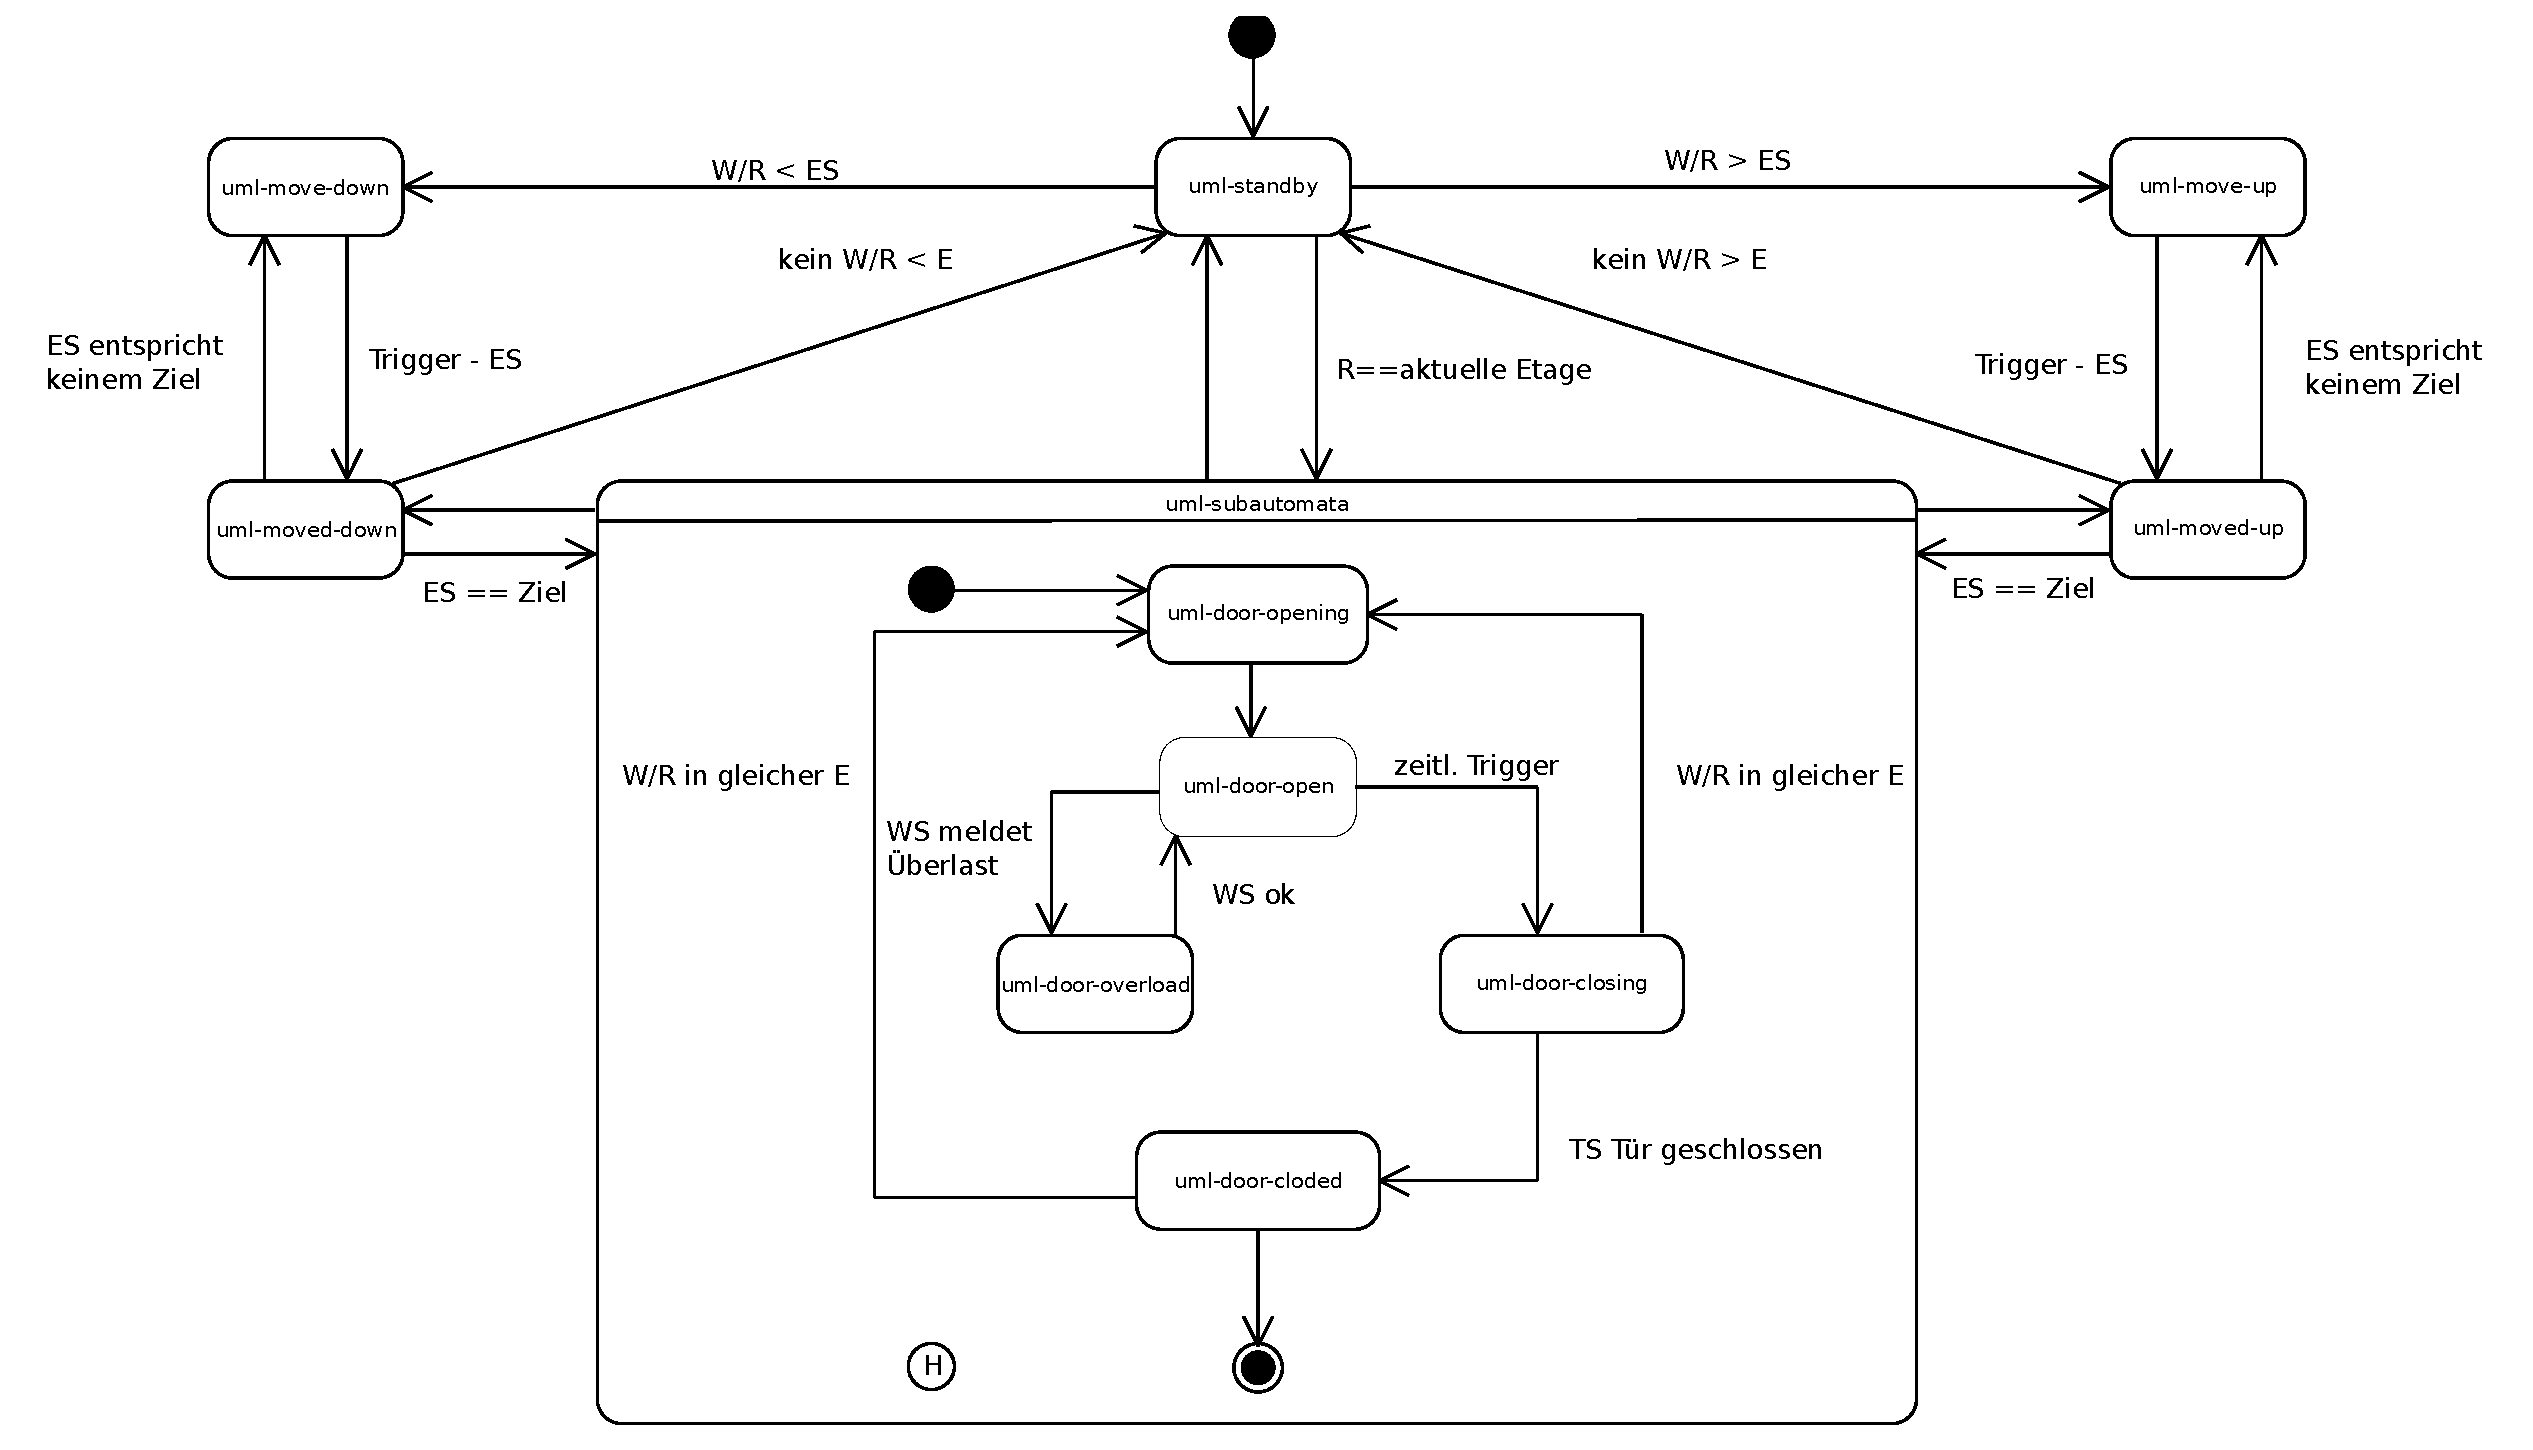
\includegraphics[width=\textwidth]{images/ZDv6_id_view.eps}
	\caption{IDs des Zustandsdiagrammes}%
	\label{fig:ZD_id_view}%
\end{figure}

\section{Erweiterungen}

